\section{使用技巧}
\label{section_skills}

\subsection{开机自启罗技软件}

罗技软件需要\textbf{\color{red}以管理员权限启动},罗技软件自带的开机自启功能无法做到这一点。较为便捷的方式是使用 Windows 自带的\textbf{“任务计划程序”}。

\begin{figure}[H]
    \Centering
    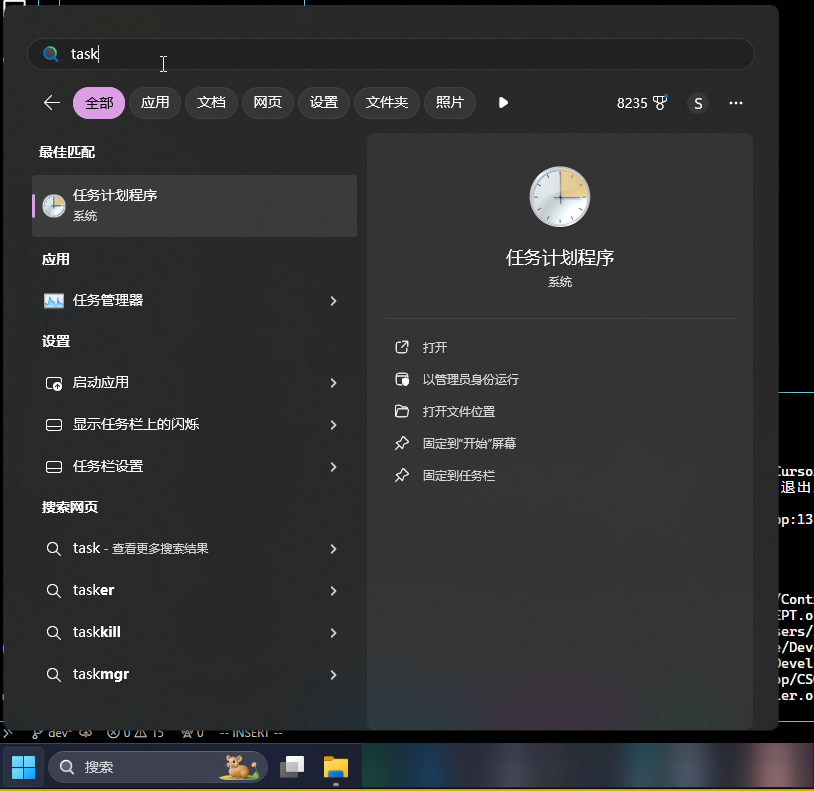
\includegraphics[width=\textwidth]{docs/assets/skills/task_scheduler.png}
    \caption{在开始菜单中搜索“task”,找到“任务计划程序”}
\end{figure}

打开后,右键“任务计划程序库”,点击“新文件夹”创建新文件夹,并为其指定名称。

\begin{figure}[H]
    \Centering
    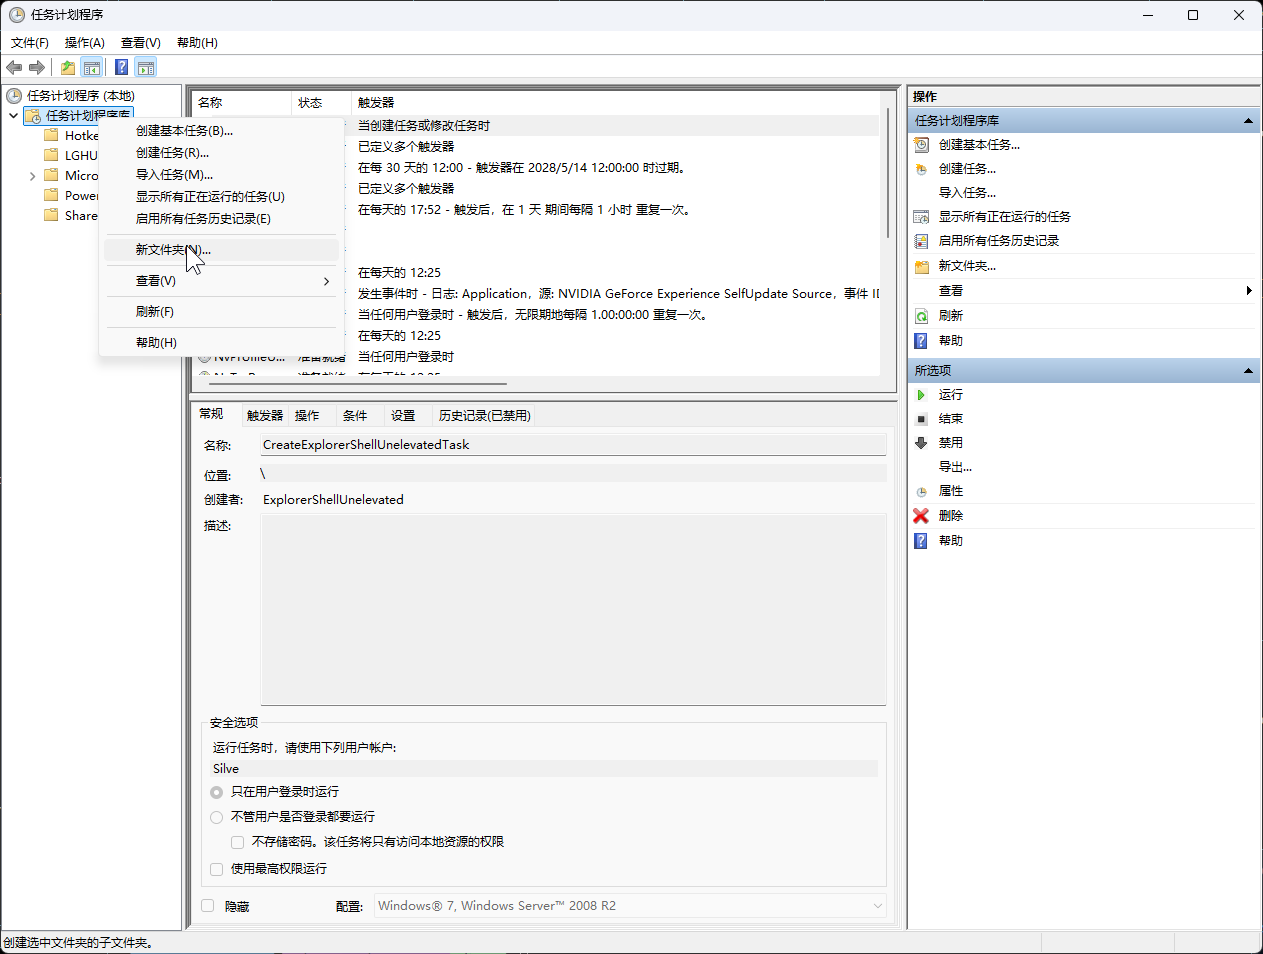
\includegraphics[width=\textwidth]{docs/assets/skills/new_folder.png}
    \caption{点击“新文件夹”}
\end{figure}

\begin{figure}[H]
    \Centering
    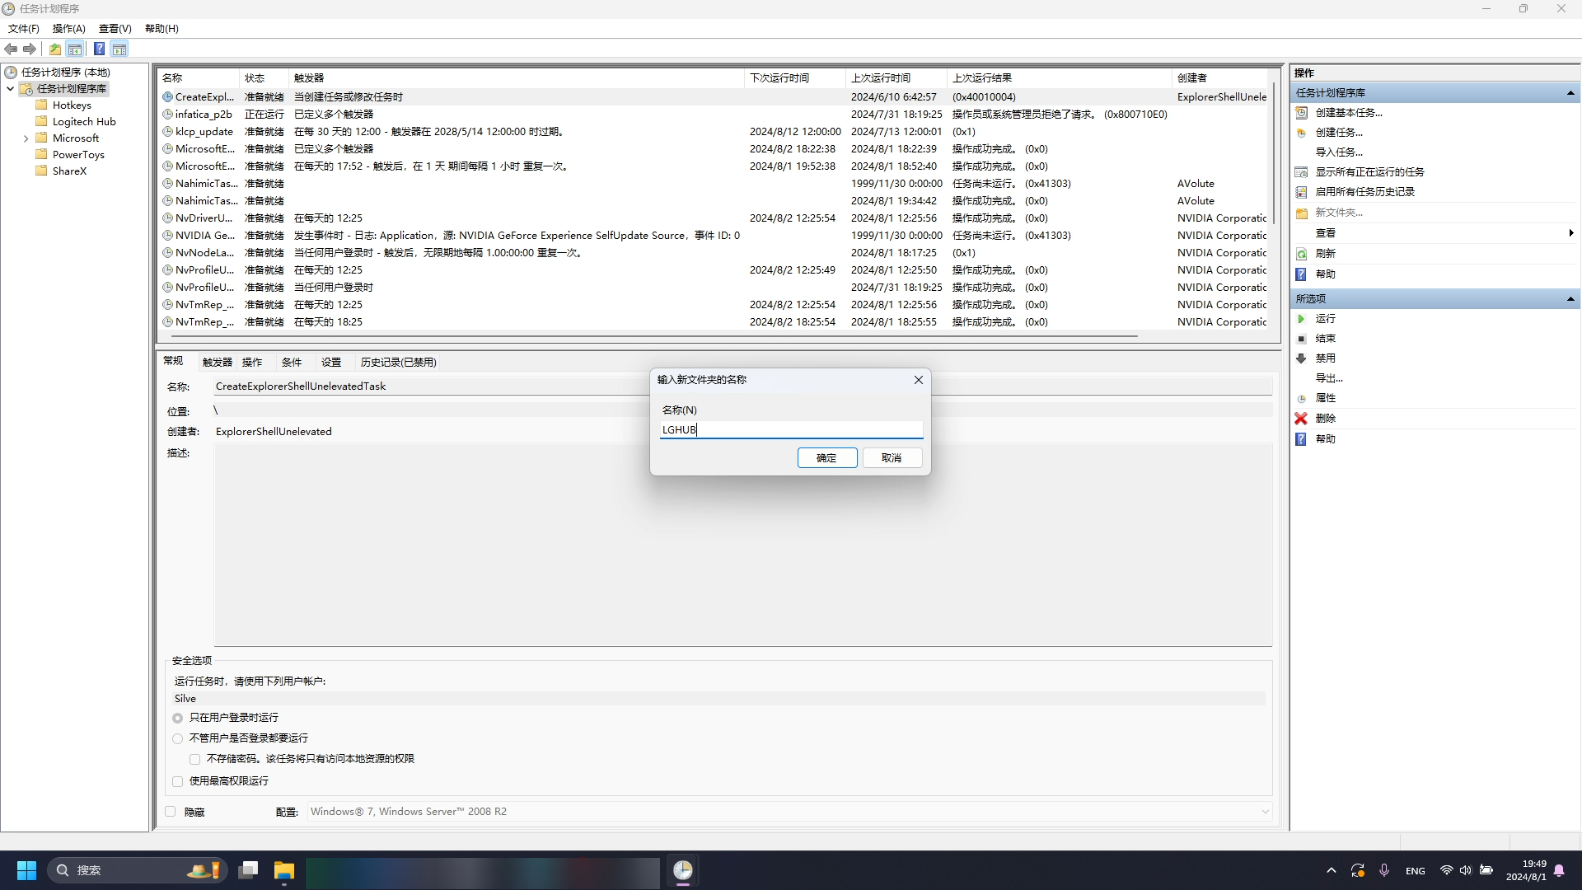
\includegraphics[width=\textwidth]{docs/assets/skills/specify_name.png}
    \caption{指定文件夹名称}
\end{figure}

右键新创建的文件夹,点击“创建基本任务”。

\begin{figure}[H]
    \Centering
    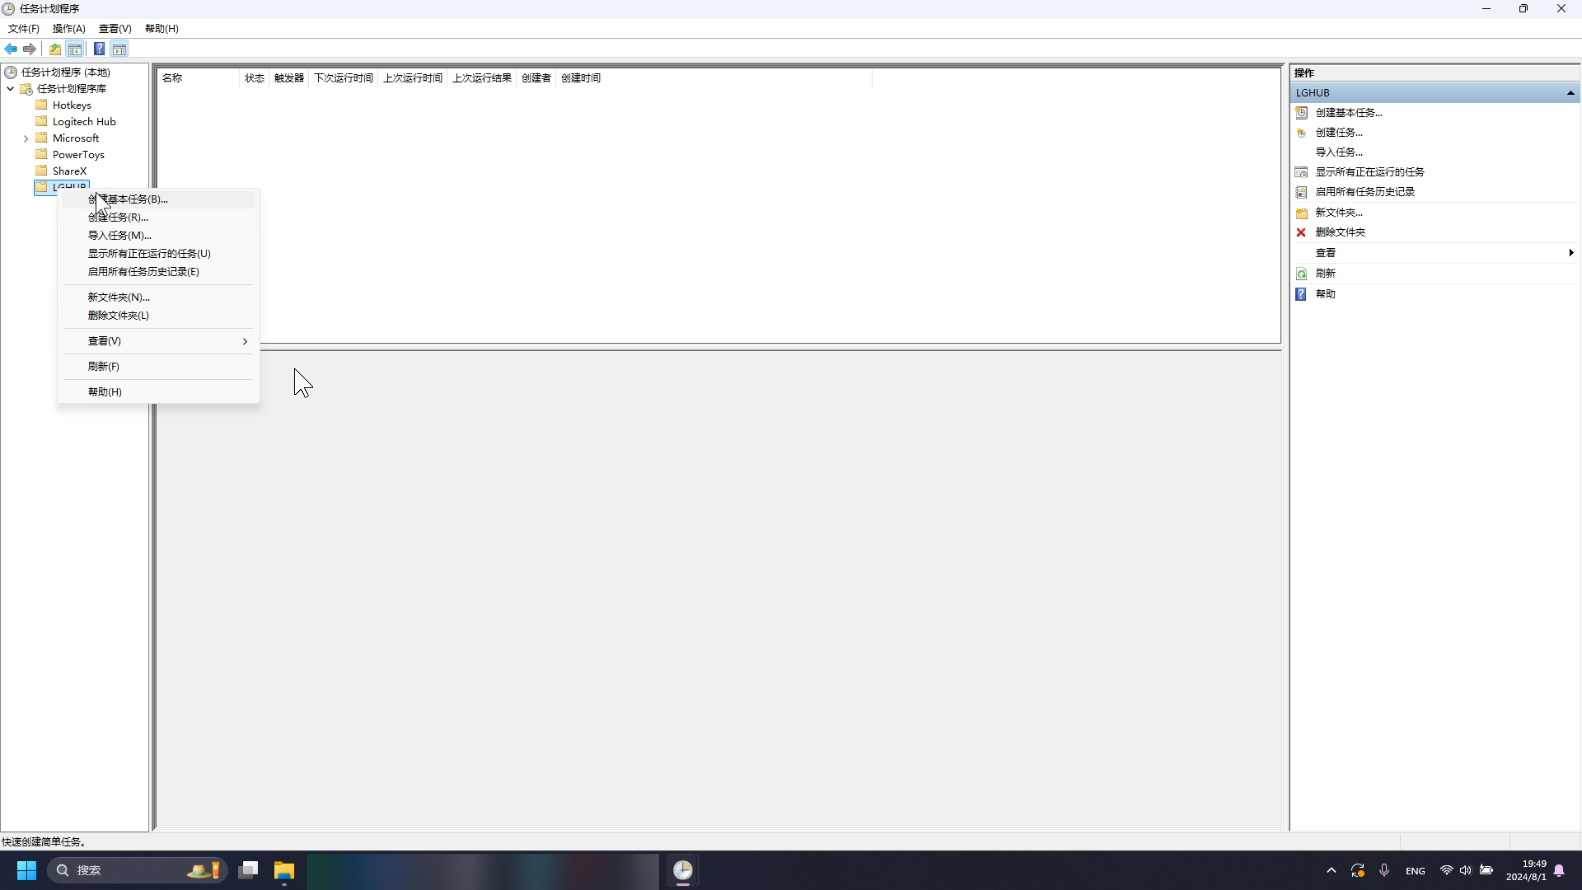
\includegraphics[width=\textwidth]{docs/assets/skills/create_basic_task_00.png}
    \caption{创建基本任务}
\end{figure}

为基本任务设置名称。

\begin{figure}[H]
    \Centering
    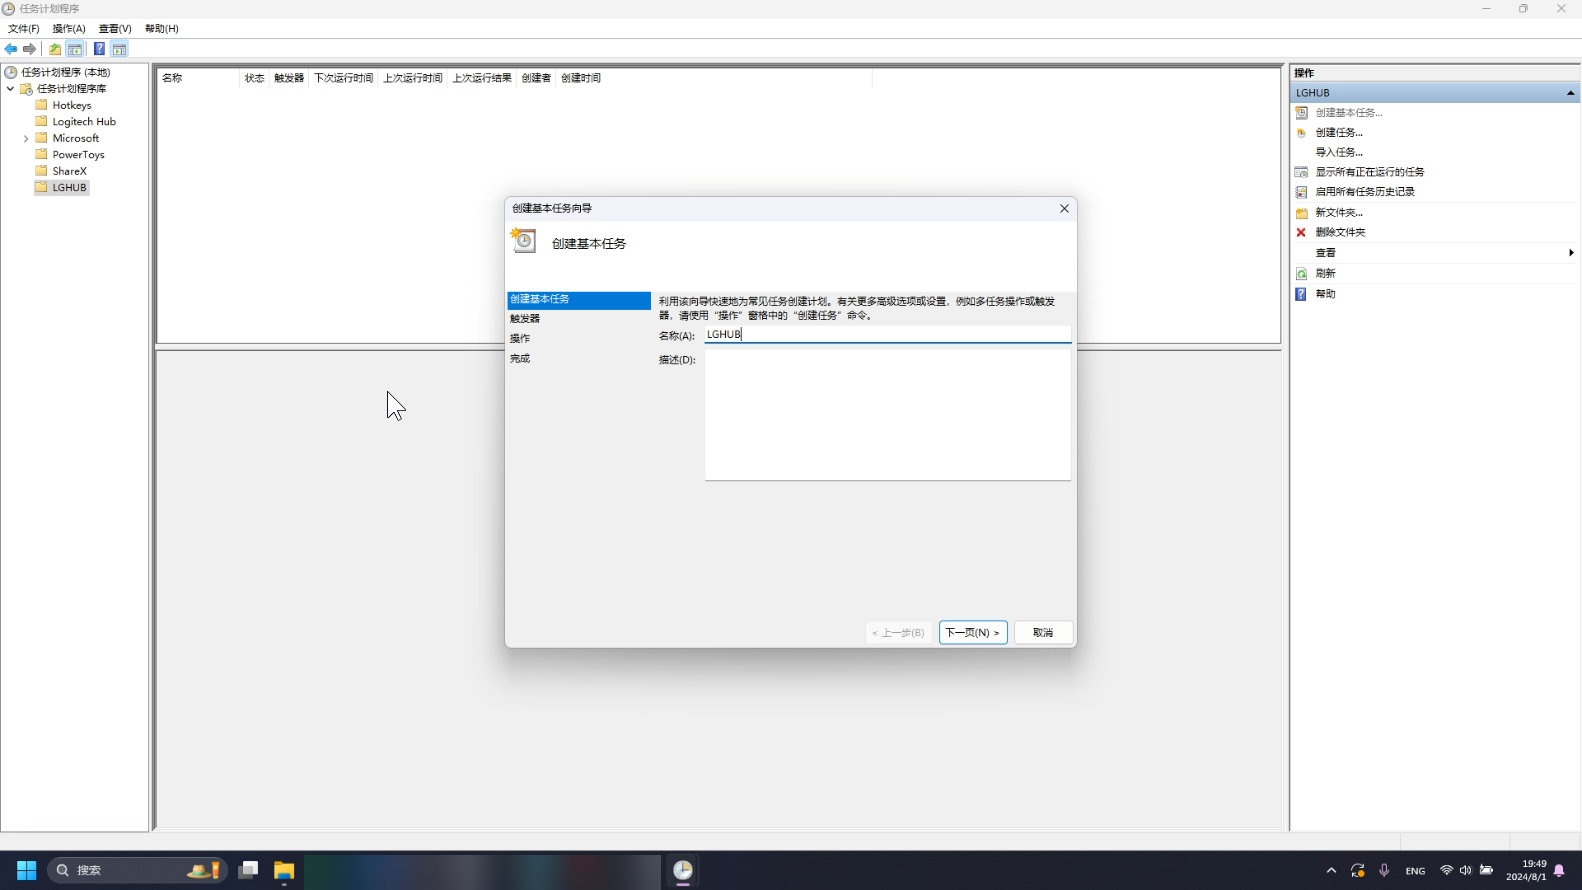
\includegraphics[width=\textwidth]{docs/assets/skills/create_basic_task_01.png}
    \caption{设置基本任务名称}
\end{figure}

触发器中设置任务在“当前用户登录时”开始。

\begin{figure}[H]
    \Centering
    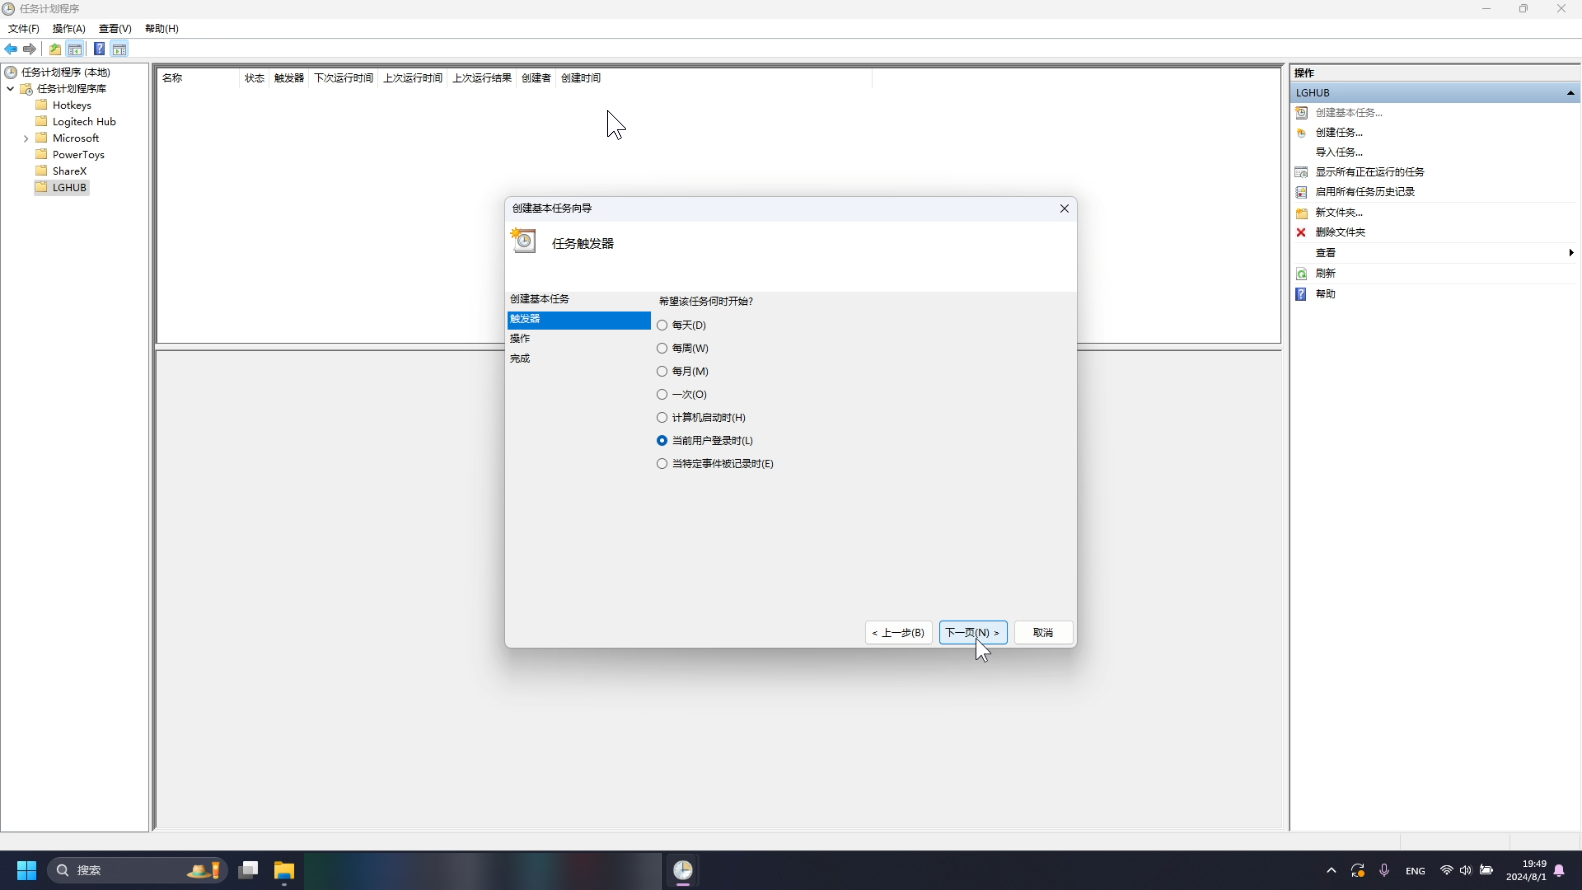
\includegraphics[width=\textwidth]{docs/assets/skills/create_basic_task_02.png}
    \caption{设置触发器}
\end{figure}

执行操作的类型为“启动程序”。

\begin{figure}[H]
    \Centering
    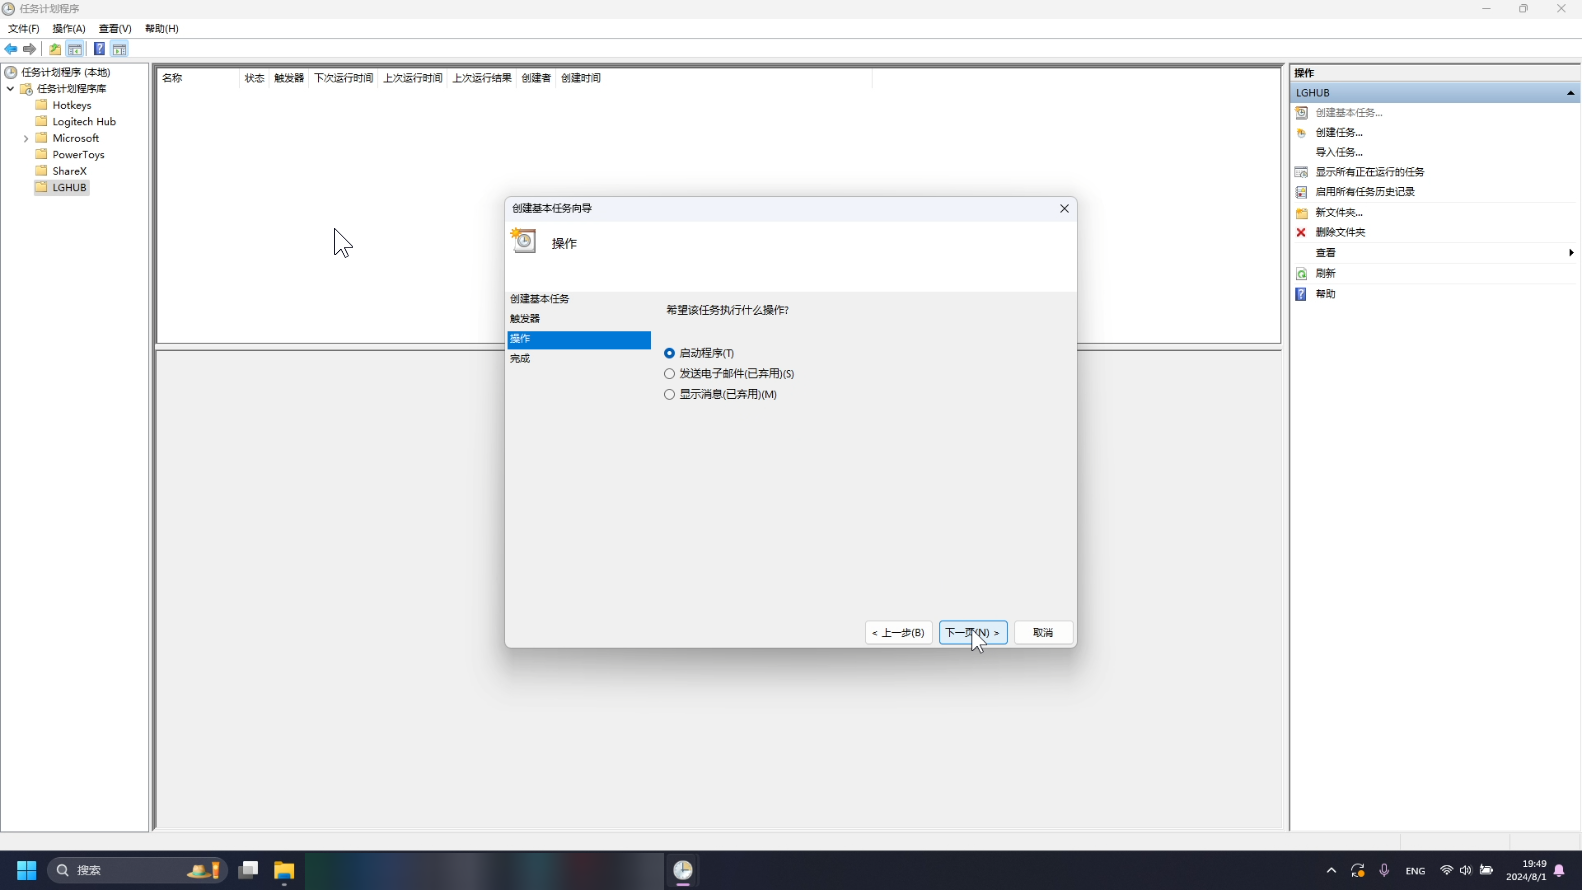
\includegraphics[width=\textwidth]{docs/assets/skills/create_basic_task_03.png}
    \caption{设置操作类型}
\end{figure}
 
然后,在桌面上右键罗技软件快捷方式,点击“属性”。

\begin{figure}[H]
    \Centering
    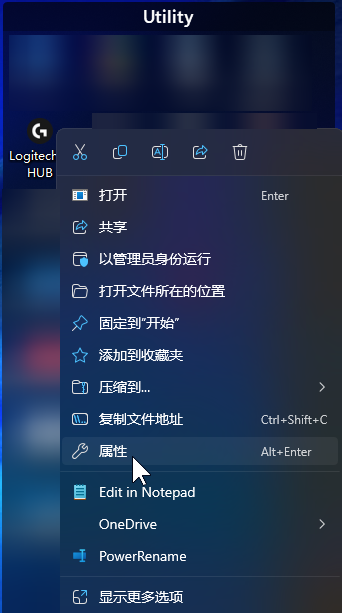
\includegraphics[width=\textwidth]{docs/assets/skills/lghub_property.png}
    \caption{点击“属性”}
\end{figure}

复制快捷方式指向的目标路径到剪切板中(\lstinline{Ctrl} \lstinline{C})。

\begin{figure}[H]
    \Centering
    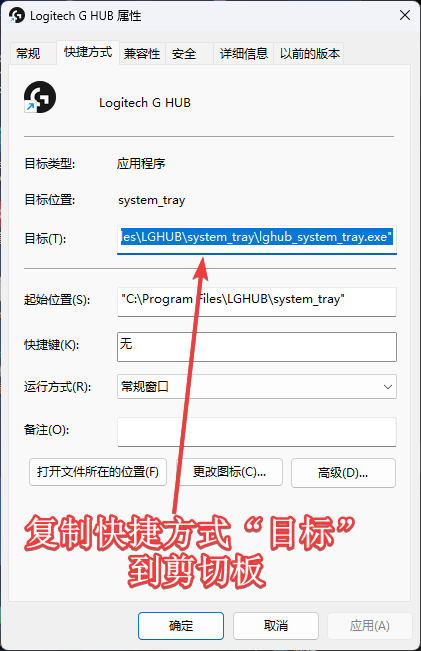
\includegraphics[width=\textwidth]{docs/assets/skills/create_basic_task_04.png}
    \caption{复制快捷方式“目标”}
\end{figure}

在“程序或脚本”一栏粘贴上述步骤复制的目标路径到地址栏(\lstinline{Ctrl} \lstinline{V})。

\begin{figure}[H]
    \Centering
    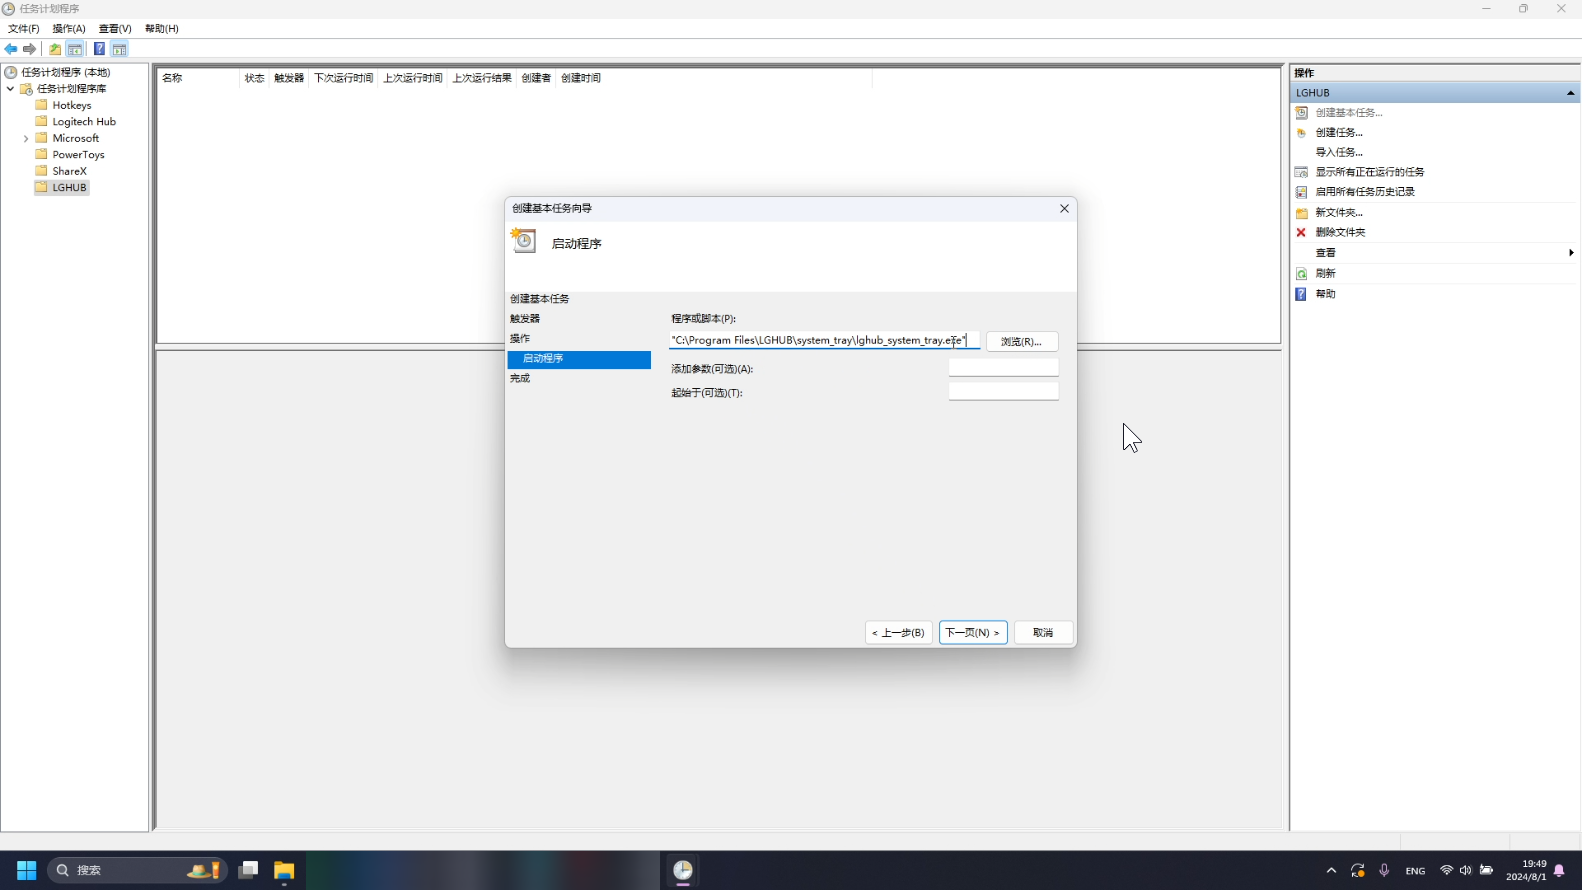
\includegraphics[width=\textwidth]{docs/assets/skills/create_basic_task_05.png}
    \caption{粘贴到地址栏中}
\end{figure}

在添加参数一栏输入 \lstinline{--background}(设置罗技软件自启时不弹出窗口,在后台静默运行)。

\begin{figure}[H]
    \Centering
    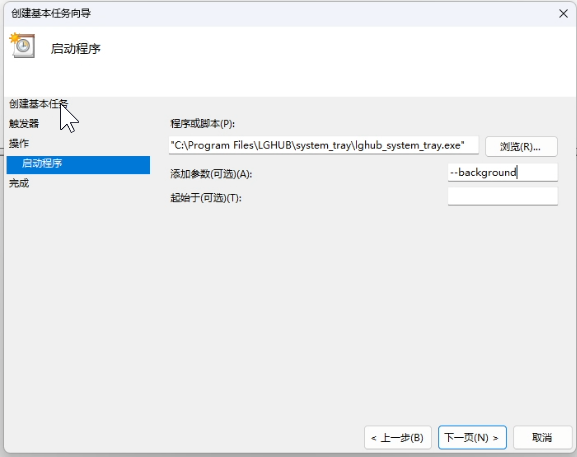
\includegraphics[width=\textwidth]{docs/assets/skills/create_basic_task_06.png}
    \caption{添加 \lstinline{--background} 参数}
\end{figure}

勾选图示选项后,点击完成。

\begin{figure}[H]
    \Centering
    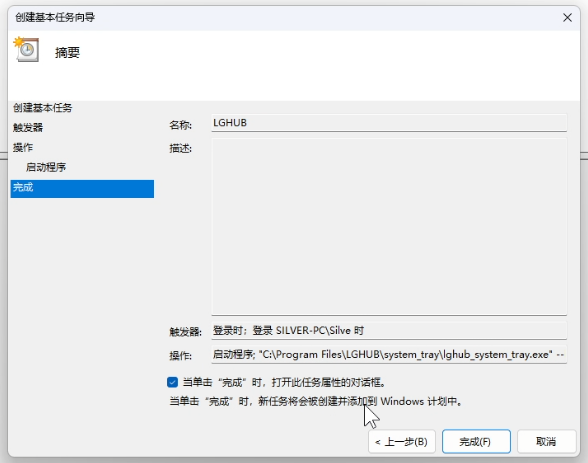
\includegraphics[width=\textwidth]{docs/assets/skills/create_basic_task_07.png}
    \caption{完成后弹出任务属性对话框}
\end{figure}

在弹出的窗口中选择“使用最高权限运行”。

\begin{figure}[H]
    \Centering
    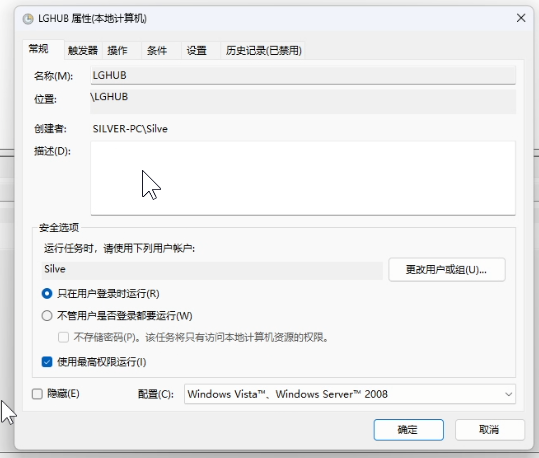
\includegraphics[width=\textwidth]{docs/assets/skills/create_basic_task_08.png}
    \caption{勾选“使用最高权限运行”}
\end{figure}

然后,点击“条件”,去除下图所示的与电源相关的任务运行条件\textbf{\color{red}(对于笔记本用户,此项必须去除,否则在笔记本使用电池电源时,任务将不会启动,启动的任务也将退出)}。

\begin{figure}[H]
    \Centering
    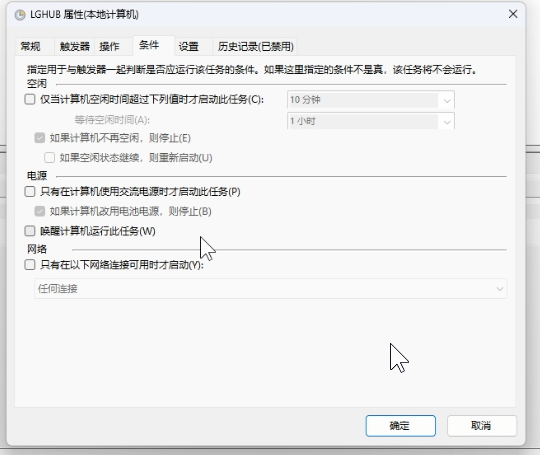
\includegraphics[width=\textwidth]{docs/assets/skills/create_basic_task_09.png}
    \caption{去除与电源相关的任务运行条件}
\end{figure}

最后,点击“设置”,去除与程序运行时间限制(如“运行时间超过 3 天停止任务”这样的选项)。

\begin{figure}[H]
    \Centering
    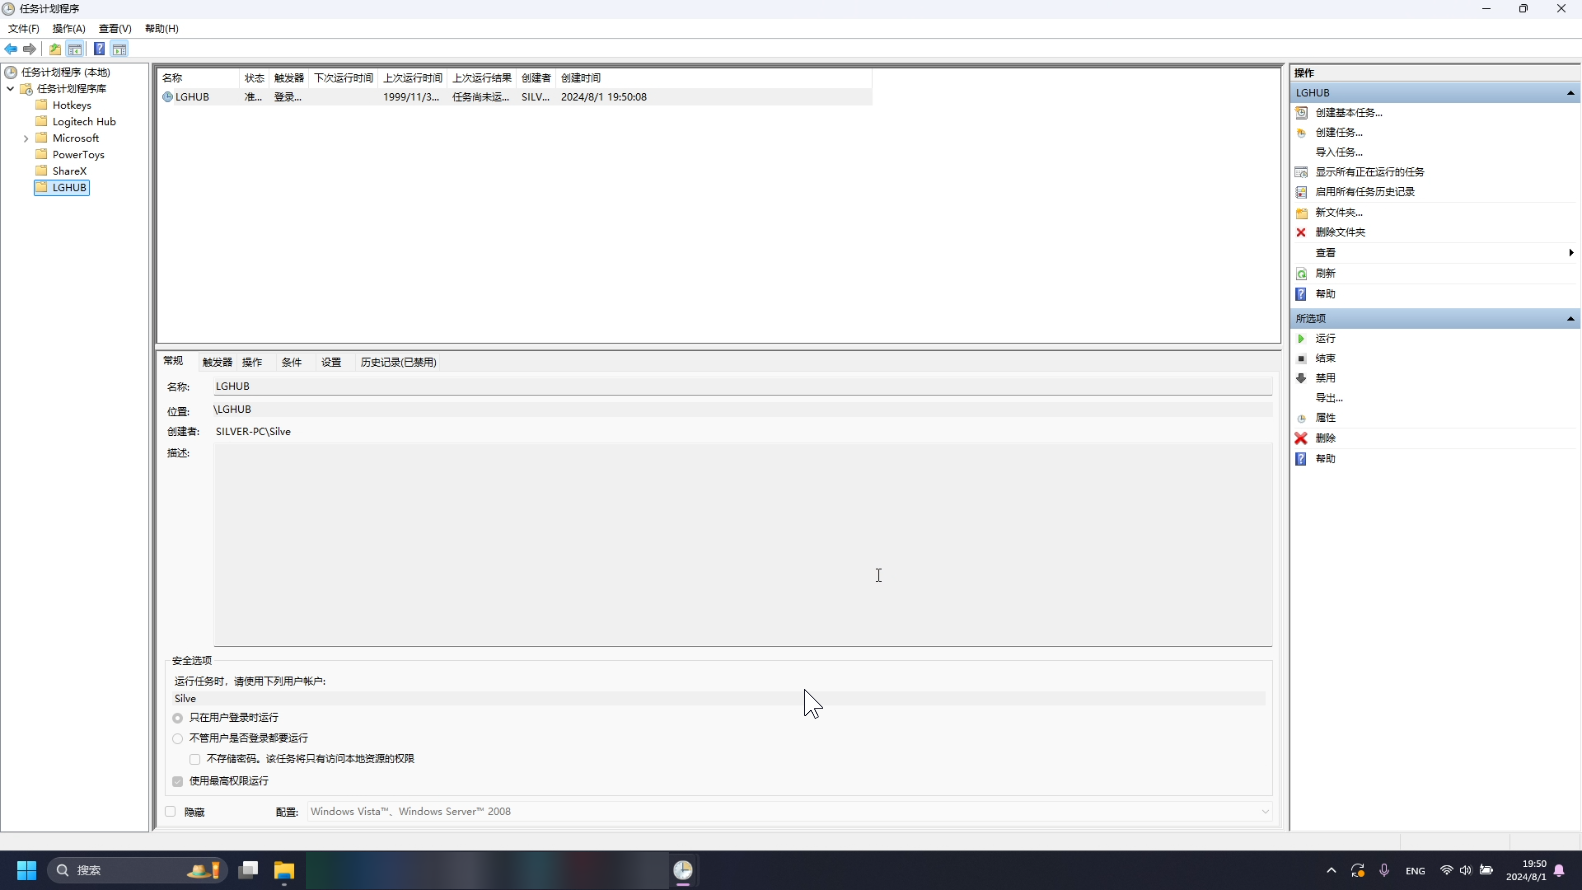
\includegraphics[width=\textwidth]{docs/assets/skills/create_basic_task_10.png}
    \caption{解除运行时间限制}
\end{figure}

点击“确定”后,可在 \lstinline{LGHUB} 文件夹中找到新创建的基本任务。下一次电脑开机并以当前用户账户登录后,罗技软件将自动以管理员权限启动。

\begin{figure}[H]
    \Centering
    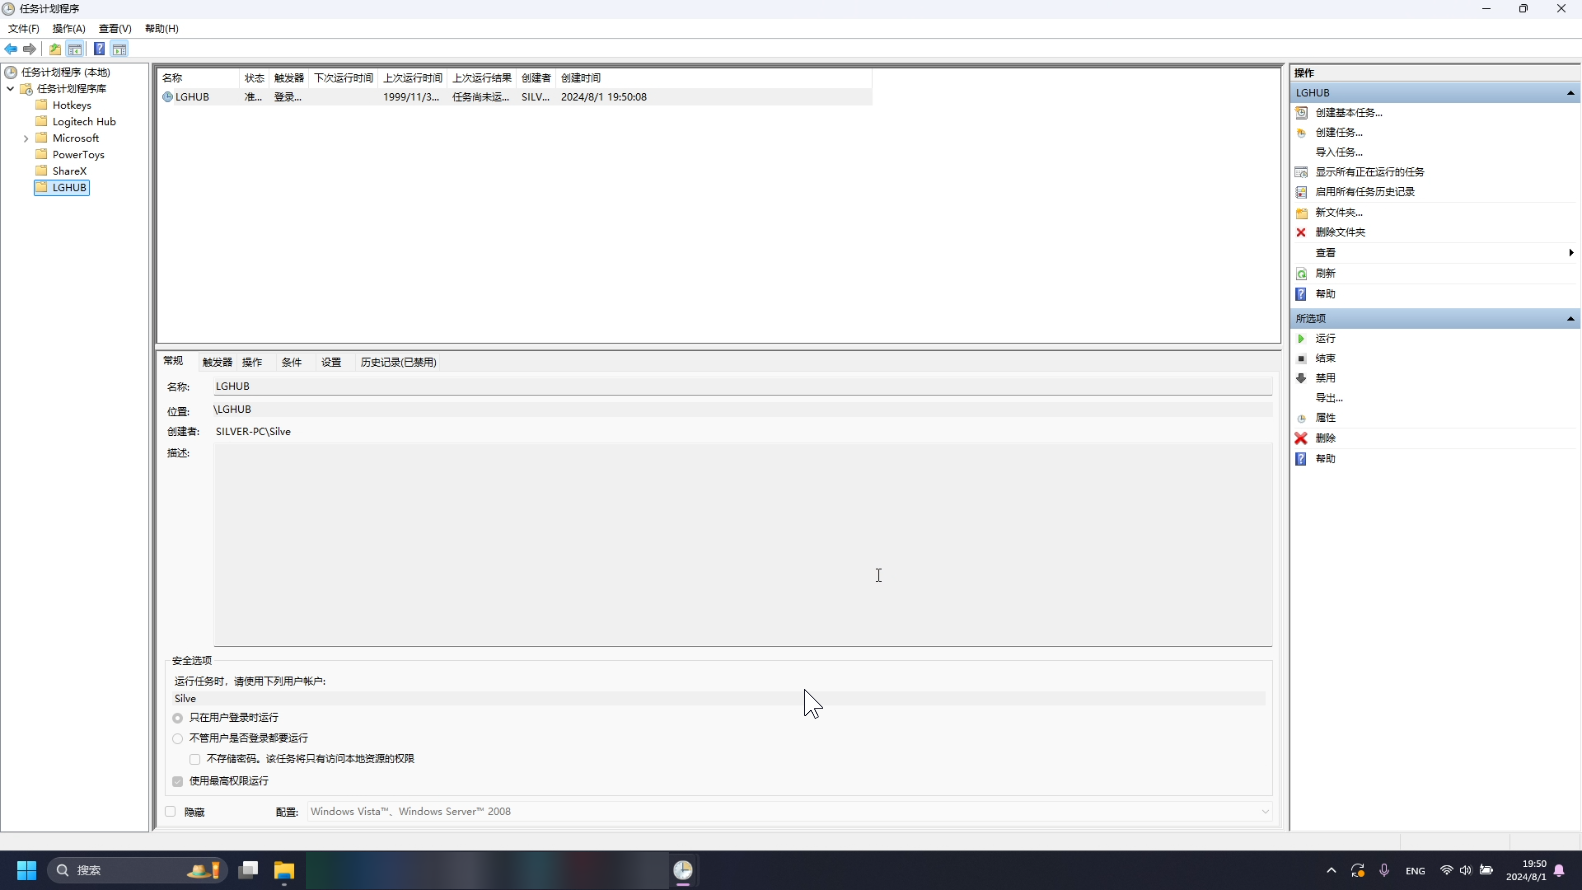
\includegraphics[width=\textwidth]{docs/assets/skills/create_basic_task_11.png}
    \caption{创建完成的基本任务}
\end{figure}

要想立即运行已经创建的基本任务,请右键该任务,点击“运行”即可(已经运行则跳过此步骤)。上述创建开机自启任务的方法同样适用于其他任何应用程序。

\begin{figure}[H]
    \Centering
    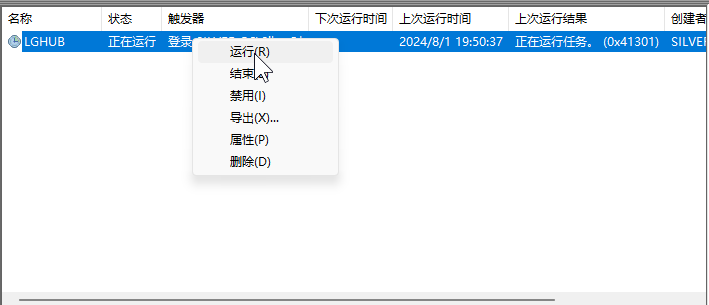
\includegraphics[width=\textwidth]{docs/assets/skills/run_task.png}
    \caption{立即运行已经创建的基本任务}
\end{figure}
